%***********************************************************************
%* File            :    titel2.tex
%*
%* Titelseite
%*
%* Autor           :    Daniel Hering
%***********************************************************************

\newcommand{\defaultarraystretch}{\arraystretch}

\begin{titlepage}
\enlargethispage{31mm}
%***********************************************************************
%* Definition der Kopfzeile																						 *
%***********************************************************************
\vspace*{-3cm}
\hspace*{-1.8em}
\begin{tabularx}{19cm}{Xl@{}}
\textsf{\textbf{\LARGE{\docsubject}}} & %
\includegraphics[height=45pt]{images/RWTH_Aachen_University}
\\
\mbox{\vspace{-10mm}\colorbox{rwthblue}{\hspace{18.4cm}}
\rule{0pt}{10pt}}
%\vspace{-10mm}\colorbox{rwthblue}{\hspace{12.7cm}}  {
\includegraphics[height=30pt]{images/medit_l_m_blau_meditheadfoot}}
\end{tabularx}

%***********************************************************************
%* Ende der Definition der Kopfzeile																	 *
%***********************************************************************
\vspace*{15mm}
\par
\begingroup
\huge
\leftskip20pt
\noindent \textsf{\LARGE\docauthor\\
\textbf{\huge \docshorttitle}}
\par
\endgroup
\vfill % F�llt die Seite vertikal auf

%***********************************************************************
%* Hier eine zur Diplomarbeit geh�rende Grafik einbinden 							 *
%***********************************************************************
% 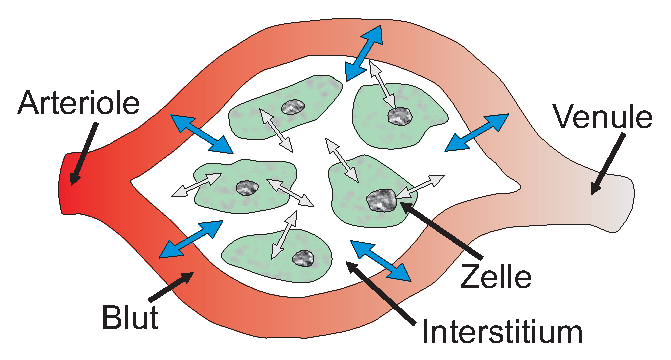
\includegraphics[width=190mm]{images/beispiel1}\vspace{10pt}
%
% \AddToShipoutPicture*{
%      \parbox[b][\paperheight]{\paperwidth}{%
%        \vfill
%         \centering
%         \begin{tikzpicture}[overlay]%
%        		  %\draw[help lines] (0,0) grid (10,20);
%             \node (0,0) [opacity=0.4]{%
%              \hspace{-8,25mm}\includegraphics[width=10cm, height=10cm,keepaspectratio]{\doctitlepic}};%
%          \end{tikzpicture}
%        \vspace{32.35em}
%      }}







\renewcommand{\arraystretch}{1.3}
\hspace*{-1.8em}
\begin{tabularx}{19cm}{Xl}
\multicolumn{2}{l}{\colorbox{rwthblue}{\hspace{18.4cm}}}\\
\multicolumn{2}{l}{\textsf{\textbf{CHAIR FOR MEDICAL INFORMATION TECHNOLOGY}}}\\
\multicolumn{2}{l}{\textsf{{Faculty of Electrical Engineering and Information Technology, RWTH Aachen}}}\\
\multicolumn{2}{l}{\textsf{Univ.-Prof. Dr.-Ing. Dr. med. Dr. h.c. Steffen Leonhardt}}\\
\textsf{Supervisor: \docsupervisor} & \\
\textsf{Date: \today} & \multirow{-2}*~%{
\includegraphics[height=30pt]{images/medit_l_m_blau_meditheadfoot}} \\
\end{tabularx}%}
\renewcommand{\arraystretch}{\defaultarraystretch}

\thispagestyle{empty}
\cleardoublepage

\end{titlepage}
